\section{Fourth Part : Goal discussion} \label{part4}

\subsection{Discussion about forecasting goal} \label{goal}

Now that the comparison of the models as been done with as goal the minimization of the prediction error, as defined in sections concerning the loss \ref{loss} and the metrics \ref{metrics}, we can interrogate the pertinence of this "by default" goal in the particular context the forecast models must be used.

The third step of the stochastic decision process described in section \ref{intro} is, more than everything, interested in a forecasting that gives a precise estimation of the value of production for which there is a very low probability (value that could be discussed) that the production in the given time window outnumber this value. That value will be called the "security limit" and will be used to determine, knowing what is the maximum acceptable production value, if the generator limits must be modified.
In other terms, considering that the model output is a probability distribution, the goal fixed is not to minimize the difference (in any ways to define it) between the predicted and observed time series but to minimize the difference between the predicted "security quantile", i.e the $quantile(1-e)$ of the predicted distribution, knowing that $e$ is the probability of error considered as acceptable, and the real security quantile (the quantile of the real probability distribution of the source).
A too low predicted security quantile signify that the risk of production oversupply is underestimated,
leading to situations where the system will estimate that the network is safe wrongly. 
Inversely a too high predicted security quantile signify that the risk is overestimated, leading to situations where the production limit will be decreased unnecessarily low. This situation is nevertheless less problematic than the first one.
The minimization must be for all time steps of the prediction range. 

This objective is not disconnected from the classical objective consisting in minimizing the difference between the predicted and observed time series.
If the predicted distribution is close to the real distribution, the predicted security quantile tends to be close to the real security quantile.



\subsection{New metric}\label{other_metrics}

Knowing the goal pursued (\ref{goal}), the metric must indicates if the predicted quantiles are over/under-estimated. 
The defined objective (\ref{goal}) cannot be expressed literally as the quantiles of the real distribution are unknown.
The proposed 
metric, \textit{Coverage} uses an implemented metric, $coverage$.
This metric is defined as, taking as argument \textit{N} randomly drawn sample values of the predicted probability distribution ($[{x_1},...,{x_N}]$), one observed value y,
q the quantile considered and $quantile_q([{x_1},...,{x_N}]$ a function giving the quantile q value for the approximated distribution constructed on the samples $[{x_1},...,{x_N}]$ :

\begin{equation}
    coverage(q,y,[{x_1},...,{x_N}]) = \frac{1}{N}\sum_{i=0}^{N} \mathbb{I}(y<quantile_q([{x_1},...,{x_N}])
\end{equation}


This metric gives the observed probability having a value below the quantile q.

The Coverage metric is defined as, for $e$ is the probability of error considered as acceptable  :  
\begin{equation}
%Coverage = (0.01 - coverage(0.005)) + (coverage(0.995) - 0.995) 
    Coverage(q,y,[{x_1},...,{x_N}]) = coverage(1 - e,y,[{x_1},...,{x_N}]) - (1 - e)
\end{equation}

The Coverage of the predicted distribution must tends to 0 to achieve the goal. For the upper quantile,
if coverage(x) > x, the quantile is too high (the window is too large) and
if coverage(x) < x the quantile is too tight.

This metric is not sufficient to evaluate the quality of a model prediction. The model could have a good Coverage value because the predicted probability distribution is very spread out. 

Another useful indicator is how much the output probability distribution is spread out. 
Between two models with a Coverage of 0, the best model is the one which gives the thinner probability distribution, or in other terms, the lesser difference between the security quantile and the median.
A proposed metric is  the mean of the difference between 
the $quantile(1-e)$ and $quantile(e)$ values. We could use $quantile(0.5)$, the median, instead of $quantile(e)$. For a time series :

\begin{equation}
    Bandwidth(y,[{x_1},...,{x_N}]) = \frac{1}{T}  \sum_{t=0}^{T-1} quantile_{1-e}([{x_1},...,{x_N}]) - quantile_e([{x_1},...,{x_N}])
\end{equation}


\subsection{Custom Loss} \label{custom_loss}
Considering that, as we have seen in section \ref{goal}, the model training must follow an non-traditional goal, the loss function must be discussed.
The loss must take account if the predicted quantiles are over/under-estimated.

The loss could be equivalent to the metric Coverage described in section \ref{other_metrics}.

We could also use a different loss that penalize values of x bigger than $quantile(1-e)$
This proposed loss, which is non binary on the contrary to the metrics, is the following, for $\phi(x)$ is the output density distribution and y the observed value  :

\begin{equation}
    %alt\_loss(x,\varphi ) = e^{x - quantile_\varphi (0.995)} + e^{quantile_\varphi (0.005)-x}
    alt\_loss(y, \phi(x) ) =  e^{y - quantile_{1-e}(\phi(x))} 
\end{equation}


The loss increase exponentially if x superior to the security quantile, and is remains low if not.

%This loss express indirectly the objective that has been fixed, by penalising heavily the model when observed values overcome the security quantile, indicating that the quantile is too low. 
%The opposite situation (window too large) is handle by the base loss, as this situation results in a higher loss, in mean.
%See \ref{fig:distrib_comp}.


The only way to use other loss than the default loss in GluonTS is to define custom models, based on the original but with intern modifications to change loss function.

4 custom models (one original, \textit{"Simple"}, and the copy of the pre-implemented \textit{"SimpleFeedForward"} and 
\textit{"CanonicalRNN"}, \textit{DeepAr}) are implemented. 

Some models are different and cannot use another loss, some cannot use the defined custom loss because of implementation problematics, notably because in the current version of GluonTS the use of a custom model implies that the hybridisation, important part of the implementation optimization, cannot be used, resulting in very important training time.

The loss implemented in these custom model is the following :

\begin{equation}
    custom\_loss(x,\phi ) = base\_loss(x,\phi ) + \alpha * alt\_loss(x,\phi )
\end{equation}



\begin{figure}[!h]
    \centering
    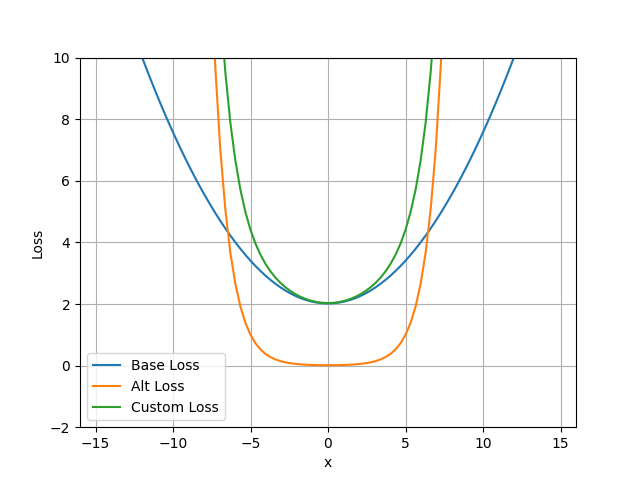
\includegraphics[width=400px]{base_loss_vs_custom_loss.png}
    \caption{Comparison of Base Loss, Alt Loss and Custom Loss, with x the difference between the observed value and
    the median of the predicted distribution}
    \label{fig:customloss}
\end{figure}

With $\alpha$ an hyper parameter, It value is a subject of a study in section \ref{comp2_alpha}.



